\documentclass[12pt, A4]{report}

\usepackage{amsmath}
\usepackage{amssymb}
\usepackage{arydshln}
\usepackage{bm}
\usepackage{csquotes}
\usepackage[hang,flushmargin]{footmisc} 
\usepackage[margin=0.5in]{geometry}
\usepackage[utf8]{inputenc}
\usepackage{imakeidx}
\usepackage{moresize}
\usepackage{multirow}
\usepackage{pgfplots}
\usepackage[shortlabels]{enumitem}
\usepackage{tikz}
\usetikzlibrary{calc}

\DeclareMathOperator{\df}{\mathrm{df}}
\DeclareMathOperator{\ME}{ME}
\DeclareMathOperator{\nint}{nint}

\newcommand{\Chi}{X}
\newcommand{\cint}{\text{confidence interval}}
\newcommand{\diff}[1]{#1_{\mathrm{diff}}}
\renewcommand{\Roman}[1]{\MakeUppercase{\romannumeral #1}}
\newcommand{\pval}{P\text{-value}}
\newcommand{\z}[3]{\frac{#1 - #2}{#3}}

\title{Review}
\author{Arnav Patri}

\begin{document}
	\maketitle
	\tableofcontents
		\chapter*{Topic 1: Sampling Techniques and Sources of Bias}
			\addcontentsline{toc}{chapter}{Topic 1: Sampling Techniques and Sources of Bias}
			\begin{enumerate}
				\item 
					Know and understand the difference between a \emph{population} and \emph{sample}
						\begin{itemize}
							\item 
								How is each one measured? Use the proper \emph{vocab term}!
									\subitem
										A population is measured via a census while a sample is measured via a survey/experiment.
							\item
								Why do we often measure samples instead of populations?
									\subitem
										It is often infeasible to collect data from every member of a population.
						\end{itemize}
				\item
					Know the different types of \emph{bias} and how to spot them in different situations
						\begin{itemize}
							\item
								What is the difference between \emph{sampling error} and \emph{sampling bias}?
									\subitem
										Sampling error is unrepresentativeness as a result of the fact that a sample is being taken rather than a census. As	the sample is never going to exactly represent the population, it is unavoidable, but it can be mitigated by a larger sample or a more representative sampling technique. Sampling bias is the systematic skewing of results away from the true population results as a result of fault inherent to the sampling procedure.
							\item
								How can a small sample size affect the validity of the sample? (\emph{this is related to sampling \underline{error} rather than bias})
									\subitem
										The smaller the sample, the greater the likelihood of it misrepresenting the full population, simply because it is difficult to get a full picture from only a few data points. It is also more likely for the sample to be unrepresentative of the population due to pure chance.
						\end{itemize}
			\end{enumerate}
			\[\begin{tabular}{|p{9cm}|p{9cm}|}\hline
				Define the types of \textbf{\underline{sampling bias}} (a bias in \emph{who} was in the sample) &
				Define the types of \textbf{\underline{response bias}} (a bias in \emph{what} the sample is saying). \\\hline
				\textbf{Under-coverage bias} is bias caused by certain subsets of the population being underrepresented in the sample. &
				\textbf{Loaded questions} may be difficult for respondents to answer fully or truthfully, introducing bias. \\
				\textbf{Nonresponse bias} is bias as a result in certain subsets of the population choosing not to participate in the sample despite being selected. &
				\textbf{False answers} may be incentivized by the sample, resulting in the results being skewed. \\
				\textbf{Voluntary response bias} is bias as a result of only those choosing to participate in a survey doing so. \\\hline
			\end{tabular}\]
			\[\begin{tabular}{|p{9cm}|p{9cm}|}\hline
				\textbf{Simple random sample:} Every member in a population should be equally likely to be chosen for the sample for it to be a simple random sample. &
				\textbf{Stratified random sample:} The population of interest should be divided into strata such that the strata are heterogenous without but homogenous within. Simple random samples should then be taken from each stratum. \\ &
					\emph{*Stratifying will \textbf{reduce variability} of possible sample results!} \\\hline
				\textbf{Systematic random sample:} Every member in a population should be assigned a number and a number. A random starting number should be selected and every $k^{\mathrm{th}}$ person (such that $k = N/n$) should be chosen. &
				\textbf{Cluster sample:} A simple random sample should be taken and those close in proximity to those selected should also be included in the sample. \\\hline
				\textbf{Multistage sample:} A simple random sample of large groups should be taken and simple random samples of those selected should be used in the sample. &
				\textbf{Convenience sample:} Those that are convenient to sample should be sampled.
			\end{tabular}\]
				\paragraph{Example:} A principal wants to create an advisory committee of 20 randomly-selected students out of the 1,800 students their high school. Describe how he could do so using a$\ldots$
			\[\begin{tabular}{|p{9cm}|p{9cm}|}\hline
				\textbf{Simple random sample:} Every student at the high school could be assigned a number from 0 to 1799, assigned alphabetically by last name. 20 non-repeating integers between 0 and 1799 (inclusive) could then be randomly generated using software. Those whose could then be assigned to the committee. &
				\textbf{Systematic random sample:} Every student at the high school could be assigned a number from 0 to 1799, assigned alphabetically by last name. Software could then be used to generate a random number from 0 to 89 (inclusive). In addition to the person whose number was initially selected, every $20^{\mathrm{th}}$ person could be selected for the committee. \\\hline
				\textbf{Stratified random sample:} Within each grade, each student could be assigned a number from 0 to $n - 1$ (where $n$ is the number of students in the grade). Software could then be used to randomly select 5 numbers between 0 and $n - 1$ (inclusive), and those whose numbers were selected could be added to the committee. This process could be repeated for each grade. &
				\textbf{Cluster sample:} \\\hline
				\textbf{Multistage sample:} &
				\textbf{Convenience sample:} The first 20 students that the principal sees could be selected for the committee. \\\hline
			\end{tabular}\]
		\chapter*{Topic 2: Experimental Design}
			\addcontentsline{toc}{chapter}{Topic 2: Experimental Design}
			\begin{enumerate}
				\item
					Know the vocabulary of experiments and experimental design
						\begin{itemize}
							\item
								What is the difference between an Experiment and an Observational Study? Which one lets us establish cause-and-effect relationships? \emph{\textbf{HINT:} There is one \emph{dead giveaway} keyword when identifying an experiment. It starts with the letter A}
									\subitem
										An experiment deliberately attempts to alter the results of those being experimented on while an observational study simply aims to observe. The former enables causality to be justified.
							\item
								Define \emph{Treatment} --
									\subitem
										A treatment is something imposed by those performing the experiment onto those being experimented on in an attempt to affect the results. 
							\item
								Define \emph{Experimental Units} (\emph{Subjects} when human) --
									\subitem
										The experimental units are the things that the data is being collected on.
						\end{itemize}
				\item
					Know the four principles of a good experiment
						\begin{itemize}
							\item
								Why is it important to \emph{randomize} the assignment of treatments?
									\subitem
										If treatments are not randomly assigned, causality cannot be justified, as there may be some other variable resulting in the responses.
							\item
								Why is \emph{comparison} (either with a control group OR a second treatment group) important?
									\subitem
										Without a comparison, there is no way of knowing whether or not the data is significant.
							\item
								In experiments, it is important to \emph{control} for outside factors or variables. What does this mean?
									\subitem
										Any variables that may affect results should be either mitigated or accounted for in the assignment process.
							\item
								What is \emph{replication}, and how can we make sure our sample has it?
									\subitem
										For an experiment to be replicable, repeated trials must be possible and produce the same results from the same initial conditions. If an experiment is not replicable, its claims cannot be corroborated, making it more likely that the results were due to sheer chance.
						\end{itemize}
				\item
					Know methods for \textbf{controlling} an experiment to prevent confounding
						\begin{itemize}
							\item
								Control group (what is it, and what does it allow us to do?)
								\subitem
								\emph{(\textbf{NOTE:} A \underline{control group} is NOT mandatory; it is just \underline{one way} to get \underline{comparison}, which \underline{IS} mandatory)}
									\subitem
										A control group is a group given the \enquote{default} treatment, often a placebo, so that the results can be tested against those of the groups given other treatments.
							\item
								Placebo effect --
									\subitem
										The placebo effect refers to the phenomenon of a treatment working simply because those taking it believe that it will work.
							\item
								Blind study --
									\subitem
										A blind study is one in which the subjects are unaware of which treatment they are being given.
							\item
								Double-blind study --
									\subitem
										A double-blind study is one in which both those giving and receiving the treatment area unaware of which treatment it is.
						\end{itemize}
					\item
						Know the different types of experimental design and how to identify which one is being used (as well as the \emph{advantages} and \emph{disadvantages} of each)
						\begin{itemize}
							\item
								Completely Randomized Design
									\subitem
										Every subject has an equal chance of receiving any given treatment.
							\item
								Randomized Block Design (\enquote{Blocking}) 
									\subitem
										The subjects are grouped by their attributes that may affect the response into blocks. Within each block, treatments are then randomly assigned. This mitigates confounding variables and makes comparison between treatments easier.
							\item
								Matched Pairs Design
									\subitem
										The data is paired, measuring some change in results from the same initial conditions. This ensures that any change is due only to the treatment.
						\end{itemize}
			\end{enumerate}
			\paragraph{Example:} \emph{A researcher studied a random sample of 100 teens in Oklahoma. To which populations will the results of this researcher's findings be generalizable?} (Circle ALL that apply) \\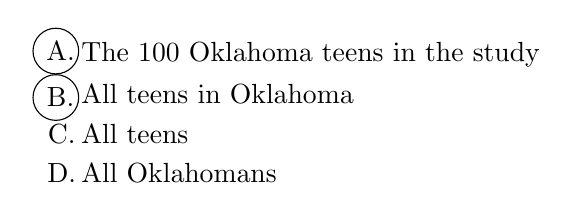
\begin{tikzpicture}
						\draw (-0.2, 0.05) circle [radius = 2.9mm] node{\hspace{1.2mm}A.};
							\node[right] at (0, 0){The 100 Oklahoma teens in the study};
						\draw (-0.2, -0.54) circle [radius = 2.9mm] node{\hspace{1.2mm}B.};
							\node[right] at (0, -0.5){All teens in Oklahoma};
						\node[] at (-0.125, -1){C.};
							\node[right] at (0, -1){All teens};
						\node[] at (-0.125, -1.5){D.};
							\node[right] at (0, -1.5){All Oklahomans};
					\end{tikzpicture}
		\chapter*{Topic 3: Analyzing Data}
			\addcontentsline{toc}{chapter}{Topic 3: Analyzing Data}
			\begin{enumerate}
				\item
					The 5 things you should discuss when analyzing a \textbf{\underline{distribution}} of data:
						\begin{itemize}
							\item
						\end{itemize}
					\subitem
						\emph{\textbf{NOTE:} if asked to \underline{compare} data sets, make sure you explicitly \underline{compare} them, not just describe both of them (For example, \enquote{The first distribution has a greater mean that than the second distribution, while the second distribution has a greater spread than the first.}}
				\item
					\textbf{Center}
					\subitem
						\emph{What does it tell us about our data?}
						\subitem
							The center identifies where the data is centered, giving us the expected value of the variable.
					\[\begin{tabular}{|p{2.7cm}|p{5cm}|p{6.12cm}|}\hline
						\emph{Measure} & \emph{How to find it} & \emph{Resistant to the effects of outliers?} \\\hline
						Mean \begin{tabular}{p{2.5cm}}
							\emph{Population: $\mu$} \\
							\emph{Sample: $\bar{x}$}
						\end{tabular} &
						{\begin{align*}
							\bar{x} &= \frac{\sum x_i}{n} & \mu &= \frac{\sum x_i}{N} 
						\end{align*}} &
						\[\text{No}\] \\\hline
						
					\end{tabular}\]
			\end{enumerate}
		\chapter*{Topic 4: Normal Distributions and $Z$-Scores}
			\addcontentsline{toc}{chapter}{Topic 4: Normal Distributions and $Z$-Scores}
			\begin{enumerate}
				\item
					\begin{itemize}
						\item
							\emph{THEORETICAL}  distribution (in reality, we consider data to be approximately normal)
						\item
							
					\end{itemize}
			\end{enumerate}
\end{document}